\chapter{Økonomi} \label{Okonomi}
Formålet med dette afsnit er ud fra et økonomisk aspekt at vurdere om en given teknologisk løsning er værd at implementere i praksis. I dette tilfælde gøres det ved at benytte omkostningsminimeringsanalyse. Den benyttes under antagelse af, at den sundhedsmæssige effekt er ens i den nuværende situation og i den fremtidige situation, hvor Ultralyds Robotarmen implementeres som en add-on løsning til eksisterende ultralydsudstyr. \\
Der opstilles to scenarier. Scenarie 1 er den nuværende situation på en ultralydsscannings stue, mens scenarie 2 er den fremtidige situation på en stue med en robotarm. I analysen ønskes det at klarlægge forskellene i de to scenarier, i forhold til hvilke ressource- og omkostningsforhold der er i det enkelte scenarie. 

De økonomiske forskelle mellem de to situationer er opstillet i figur \ref{ModelOkonomi}. Denne viser forskellene i, hvilke udgifter afdelingen vil have i forbindelse med ultralydsscanning af gravide uden og ved brug af Ultralyds Robotarmen. Yderligere ses det, at der en række fællesudgifter ved begge situationer. Hver situation vil blive beskrevet yderligere i henholdsvis afsnit \ref{nuvaerende} og \ref{fremtidige}. 

\begin{figure}[H]\centering
	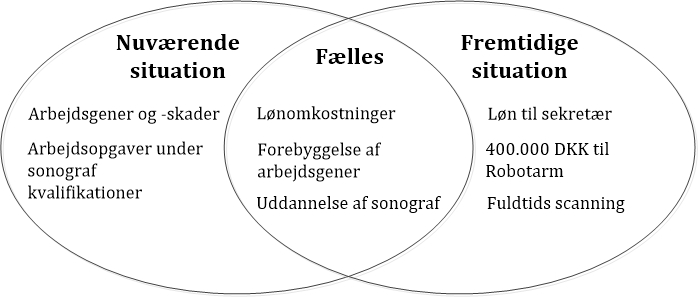
\includegraphics[width = 0.7\textwidth]{Figurer/ModelOkonomi}
	\caption{Økonomisk opdeling af udgifter i nuværende og fremtidige situation, samt fællesnævnerer}
	\label{ModelOkonomi}
\end{figure}

Belægget for dette afsnit er skabt på baggrund af interview med ”Kvindeafdelingen, Svangre- og Ultralydsambulatorium” på Hospitalsenheden Horsens (HEH), se Bilag 4. Her er deres arbejdsgange og arbejdsforhold blevet klarlagt. Se kapitel \ref{Organisation} for yderligere beskrivelse heraf. Dermed er det vigtigt at pointere, at de praktiske forhold skal være sammenlignelige med HEH førend, der kan konkluderes tilsvarende for andre afdelinger.

Yderligere tager analysen udgangspunkt i, at CEO Søren Pallesen hos Robotic Ultrasound Aps forventer, at salgsprisen på robotarmen med tilbehør bliver 400.000 DKK, se Bilag 6. \\
Scenarie 2 vil primært bygge på hypoteser, da robotten ikke er færdigudviklet endnu. \\
Grundet at robotarmen er en add-on løsning til det eksisterende ultralydsudstyr, er priser på indkøb og vedligehold af ultralydsudstyret ikke medtaget i denne analyse, da det antages at være ens i begge scenarier og dermed ikke en forskel. Alle priser i de følgende beregninger er angivet uden moms. Udgifter til service og vedligehold af ultralydsudstyret er ikke medtaget i denne analyse. 

\section{Scenarie 1 - Den nuværende situation} \label{nuvaerende}
I dette scenarie fokuseres der på omkostnings- og ressourceforbruget for at holde en ultralydsscanningsstue i drift fem dage om ugen. I den nuværende situation scanner en sonograf fire dage om ugen, mens sonografen den femte dag varetager en række arbejdsopgaver, som sonografen, i princippet, er overkvalificeret til. Dette skyldes, at det ønskes at aflaste sonograferne i deres arbejdsforhold, og dermed mindske mængden af arbejdsgener og potentielle arbejdsskader. Denne organisering af arbejdet er et valg foretaget af afdelingens ledelse, begrundelsen herfor haves der ikke yderligere belæg for, se Bilag 4. \\ 
Omkostningerne i den nuværende situation kan opdeles i følgende punkter. Hvert punkt vil blive uddybet og argumenteret senere i afsnittet.

\begin{itemize}
\item Lønomkostninger for 1,2 sonograf
\item Arbejdsgener og -skader
\item Udgifter til forebyggelse
\item Uddannelse af flere sonografer
\end{itemize}
Lønomkostninger er i dette scenarie givet ved 1,2 sonograf. Den 1,2 sonograf er estimeret på baggrund af, at det er nødvendigt at have en hel sonograf samt 1/5 af en anden sonografs arbejdstid for at have stuen bemandet fem dage om ugen. Månedslønnen for en sonograf med 2 års erfaring med kvalifikationstillæg er på løntrin 6, hvilket giver 26.967 DKK, se Bilag 4. På årsbasis giver det en årsløn på 323.604 DKK. Lønudgifter er dermed beregnet til:
\begin{equation}
323.604 \text{ DKK}\cdot1,2 = 388.325 \text{ DKK}
\end{equation}
Det ses også, at i den nuværende organisering af arbejdsgangen er der taget hensyn til, at scanning af gravide er et belastende arbejde. Dette viser sig gennem en række omkostninger til forebyggelse af arbejdsskader og -gener. Det koster blandt andet penge, at en sonograf ikke kan scanne fuldtid, og dermed bliver nødsaget til at påtage sig opgaver, sonografen er overkvalificeret til, se Bilag 4. Det vil være omkostningsmæssigt billigere, hvis opgaverne bliver varetaget af en person, hvis kvalifikationsniveau passer dertil. Denne person vil typisk modtage en lavere løn end sonografen og dermed føre til en besparelse.

Samtidig findes udgifter til skadeforebyggelse såsom ergonomiske stole, elastik-træning, massage i arbejdstiden og wellness-konsulenter, der står til rådighed for at give sonograferne råd og vejledning om bedre arbejdsstillinger og -forhold, se Bilag 4. Det har ikke været muligt at finde tilstrækkeligt oplysninger om udgifterne hertil. Dermed er disse ikke medtaget i beregningerne. 

Yderligere er der omkostninger forbundet med uddannelse af sonografer. Uddannelse af en sonograf er estimeret til at koste 108.000 DKK, se Bilag 4. Uddannelsen foregår som mesterlære over en 16 ugers periode. I denne periode er den nye sonograf altid under vejledning af mesteren. Dermed er der dobbeltbemanding på hver scanning. Således antages det at prisen på uddannelsen er givet ved lønomkostninger til den ekstra mand i form af mesteren i de 16 uger:
\begin{equation}
27.000 \text{ DKK}\cdot4 \text{ måneder} = 108.000 \text{ DKK}
\end{equation}
Der er også forbundet omkostninger ved, at sonografen først antages at kunne foretage alle typer scanninger på egen hånd efter to år, se Bilag 4. Dermed kan der være forlængede scanningstider for den nye sonograf, såfremt vedkommende støder på ukendte scenarier og bliver nødsaget til at opsøge hjælp fra mere erfarne sonografer.

Fra et regionsperspektiv er der ikke direkte omkostninger forbundet med, at en sonograf pådrager sig en arbejdsskade grundet dårlige arbejdsforhold. Ses situationen fra et samfundsperspektiv vil det kunne føre til afledte omkostninger i form af, at personen bliver nedslidt af arbejdet og tvunget tidligt på pension. Denne persons samlede livsløn vil være lavere end en sonograf, der har været på arbejdsmarkedet et fuldt arbejdsliv. Dette fører til, at denne person vil koste samfundet penge fremfor at bidrage økonomisk til samfundet. 

Hvor stort et problem arbejdsskader er økonomisk, er svært at måle. En arbejdsskade viser sig som en smerte, men det er svært at angive smerteværdien i kroner og øre. Yderligere er det svært
at svare på om smerten fremkommer af scannings arbejdet eller af en fritidsinteresse sonografen har, se Bilag 4. Dette gør at arbejdsskader viser sig som afledte omkostninger. Det har ikke været muligt at finde konkrete tal på arbejdsskader og sygedage blandt sonografer, hvor årsagen til sygdommen kan føres tilbage til selve scannings arbejdet.  


\section{Scenarie 2 - Den fremtidige situation} \label{fremtidige}
I dette scenarie fokuseres der på de ressourcer, der vil komme i spil ved implementering af en Ultralyds Robotarm som en add-on løsning til eksisterende ultralydsudstyr. Der tages ligeledes udgangspunkt i omkostnings- og ressourceforbruget for at holde en ultralydsscannings stue i drift fem dage om ugen. I dette afsnit vil der blive trukket paralleller til scenarie 1 for at tydeliggøre, hvor omkostnings forskellene er. \\
Omkostningerne i den fremtidige situation er givet ved følgende punkter. Hvert punkt vil blive uddybet i afsnittet.
\begin{itemize}
\item 400.000 DKK til robotarm med tilbehør og stativ
\item Færre arbejdsskader og -gener
\item Færre udgifter til forebyggelse
\item Regionens ansvar for personale og arbejdsmiljø
\item Lønomkostninger
\item Uddannelse af personale til brug af robotarm
\end{itemize}
Etableringsomkostninger til robotarmen med tilbehør er estimeret til at være på 400.000 DKK, se Bilag 6.
For de fleste institutioner vil en sådan udgift være et stort udlæg, derfor er det mere relevant at fordele omkostninger over den årrække, som indkøberne afskriver teknologien over. Afskrivningsperioden er på ti år, da det er estimeret, at udstyret er forældet efter ti år. Eksisterende ultralydsudstyr afskrives ligeledes over ti år, se Bilag 4.

Fordeles etableringsomkostningerne over ti år efter annuitetsmetoden med forrentningsfaktor på 2,2 \%, se Forkortelser og formler \ref{Formler}, formel 1. Forrentningsfaktoren er estimeres til at være et gennemsnit af \textbf{inflations renten} i Danmark i 2016 og 2020 \textbf{[14] - hvad er det her?}. Årligt giver dette en omkostning på 44.998 DKK:

\begin{equation}
\left(\frac{(1+0,022)^{10}\cdot0,022}{(1+0,022)^{10}-1}\right)\cdot400.000 \text{ DKK}=44.998 \text{ DKK}
\end{equation}

Det forventes, at ved brug af en robotarm ved scanning vil belastningen på sonografen være markant sænket. Det skyldes, at sonografen ikke bliver belastet af at påføre store tryk på patienten, samt bevæge arm og skulder ud i dårlige arbejdsstillinger \cite{31}. Dette uddybes i afsnit \ref{aktoerer_organisation} under Organisation. Dermed antages det i denne analyse, at der i dette scenarie ikke vil opstå arbejdsgener eller -skader grundet scanningsarbejdet. 

Udgifterne til forebyggelse vil stadig være til stede for afdelingen, da ergonomiske stole, massage og elastik-træning stadig vil være en forbedrende faktor for sonografers arbejdssforhold. Robotarmen kan bruges til cirka 80 \% af scanningerne, hvilket viser at sonografer stadig vil blive belastet som i den nuværende situation i cirka 20 \% af scanningerne, se Bilag 12, 28.04.2016. Dermed kan afdelingen ikke se bort fra at sætte penge af til sundhedsforebyggelse og - fremmende løsninger i fremtiden.  

I det første scenarie medfører det ingen omkostninger for regionen, hvis personalet bliver arbejdsskadet og dermed sygemeldt. For samfundet vil det derimod blive en stor omkostning, grundet udbetaling af understøttelse og manglende skatte indkomst. I scenarie 2 er det lige omvendt. Regionen vil have udgiften til robotarmen på 400.000 DKK som en meromkostning, hvilket vil være et stort udlæg, hvis der udelukkende ses på tallene. Samtidig har regionen også et ansvar for dens personale og arbejdsmiljø, herunder sikkerhed og sundhed. \\
Ansvaret gør, at regionen ikke udelukkende kan fokusere på tal, men også skal medtage andre aspekter når en ny teknologi muligvis skal implementeres for at forbedre arbejdsforhold for personalet. Der lægger en forventning fra samfundet om, at regionen påtager sig ansvaret for personale og arbejdsmiljø. Således regionen på den måde bidrager til at personalet kan blive i deres arbejdsposition i flere år, og dermed går senere på pension \cite{Arbejdsmiljo} \cite{RegionAnsvar}. 

Det sidste forhold, der er medtaget i denne analyse, er forskellene i lønomkostninger. I scenarie 1 skulle der 1,2 sonograf til for at bemande en stue fem dage om ugen. I dette scenarie skal der kun skulle 1 sonograf til, da det antages, at en sonograf nu kan scanne fem dage om ugen, altså fuldtid, se Bilag 4. Dette giver lønomkostninger på årsbasis:
\begin{equation}
323.604 \text{ DKK}\cdot1 = 323.604 \text{ DKK pr. stue}
\end{equation}
De arbejdsopgaver som sonografen ikke har tid til at varetage i scenarie 2 vil eksempelvis skulle udføres af en lægesekretær. En lægesekretærs bruttotimeløn på løntrin 24 er som grundsats givet ved 159,84 DKK \cite{Lontabel}. En standard arbejdsdag er 7,4 timer \cite{Arbejdstid}. Lønudgifterne til sekretæren kan således beregnes til:
\begin{equation}
159,84 \text{ DKK} \cdot 7,4 \text{ timer} \cdot 52 \text{uger} = 61.516 \text{ DKK om året}
\end{equation}
De samlede lønomkostninger til at holde en stue i drift, hvor de samme arbejdsopgaver der blev udført i scenarie 1 er medtaget, er beregnet til:
\begin{equation}
323.604 \text{ DKK/stue} + 61.516\text{ DKK/år} = 385.120 \text{DKK/år}
\end{equation}
Behovet for færre sonografer til bemanding af én stue, vil sandsynligvis over tid føre til, at færre sonografer skal uddannes. Dette vil føre til en økonomisk gevinst for regionen, da udgifterne til uddannelse af sonografer vil blive nedsat. Dog vil der naturligvis ved implementeringen af robotarmen komme en meromkostning til uddannelse i brugen der af. Dette aspekt er ikke medtaget i beregningerne. 

\section{Perspektivering til RMV}
I forbindelse med denne mini-MTV er der også indhentet oplysninger fra RMV gennem et interview. Formålet med interviewet var at få afdækket de samme områder, der blev afdækket ved interview med HEH. 

Set fra et økonomisk perspektiv er omkostningerne til at holde en stue i drift på RMV sammenlignelige med de beskrevne for HEH, se Bilag 4 og Bilag 5. Dette viser, at denne omkostnings- og ressourceanalyse er mulig at overføre til lignende afdelinger på andre hospitaler i Danmark.

\section{Delkonklusion}
Denne gennemgang af omkostnings- og ressourceforskelle mellem scenarie 1 og scenarie 2 viser, at der er en række fordele ved scenarie 1 såvel som scenarie 2. Den afgørende faktor er det dermed op til den enkelte potentielle køber at afgøre. De største forskelle er ved mængden af arbejdsskader og -gener, lønudgifter og penge til anskaffelse af Ultralyds Robotarm. Uddannelse af sonografer i brug af udstyret vil være en udgift i begge scenarier, og bidrager derfor ikke til en betydende forskel. 

Ses der udelukkende på de direkte omkostninger vil scenarie 1 være den løsning, med mindst
omkostninger. Dette skyldes at scenarie 2 er dyrere i direkte omkostninger, da robotarmen er en
add-on, og besparelsen på 3.205 DKK mellem scenarie 1 og scenarie 2 årlige lønomkostninger ikke dækker udgiften til robotarmen på 400.000 DKK, der har en årlig afskrivelse på 44.998 DKK. \\
Medtages de indirekte og afledte omkostninger, vil scenarie 2 give mulighed for besparelser, i forhold til arbejdsskader og -gener, samt en bedre fordeling af opgaver i forhold til personalets kvalifikationsniveau.  Dette kan opveje for udgifterne til robotarmen, men vil naturligvis være afhængig af den enkelte hospitalsafdeling. Scenarie 2 giver mulighed for længere tid på arbejdsmarkedet, hvorved tidlig pension undgås, hvilket giver færre omkostninger for samfundet.

